\section{Análisis de Resultados}

\subsection{Resultados Manuales P1E0}

\subsubsection{Diagramas Escala 1:200}

\begin{figure}[H]
    \centering
    \begin{minipage}{0.32\textwidth}
        \centering
        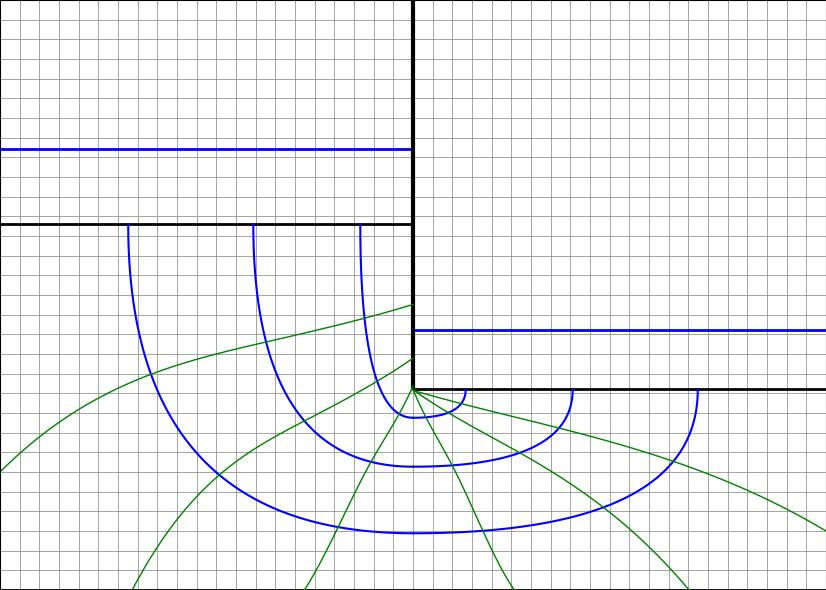
\includegraphics[width=\textwidth]{GRAFICOS/caso_1.jpg}
        \caption{Caso 1}
    \end{minipage}
    \begin{minipage}{0.32\textwidth}
        \centering
        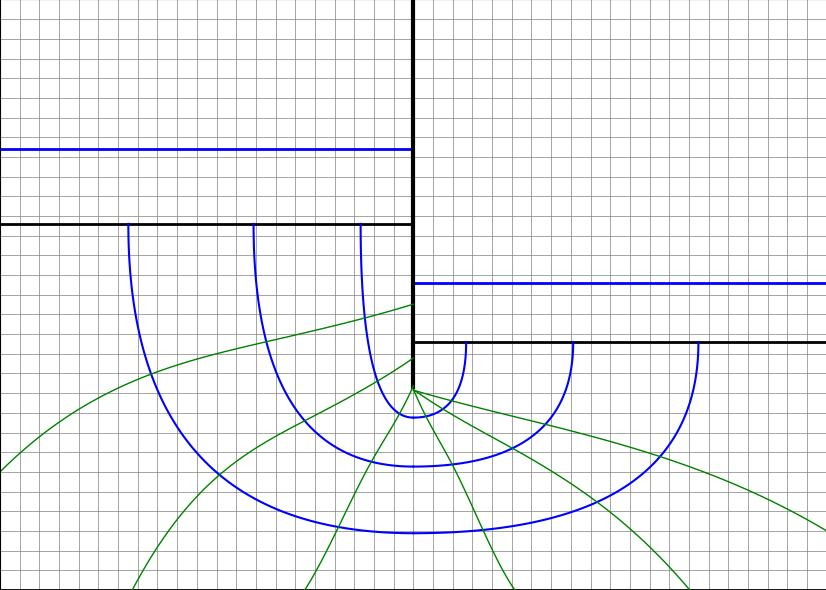
\includegraphics[width=\textwidth]{GRAFICOS/caso_2.jpg}
        \caption{Caso 2}
    \end{minipage}
    \begin{minipage}{0.32\textwidth}
        \centering
        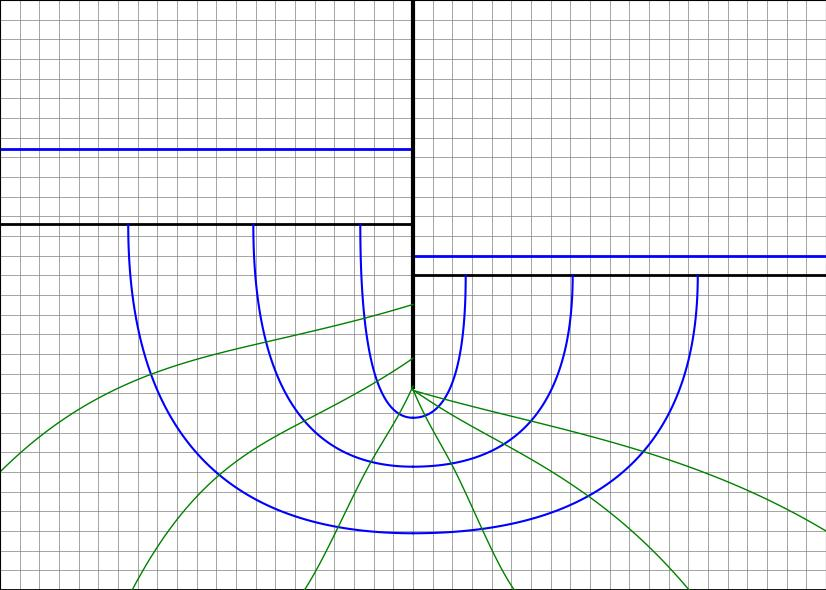
\includegraphics[width=\textwidth]{GRAFICOS/caso_3.jpg}
        \caption{Caso 3}
    \end{minipage}
  \end{figure}

\subsection{Presion de Poros}

\subsubsection{Distribucion Presiones}

\begin{figure}[H]
    \centering
    \begin{minipage}{0.32\textwidth}
        \centering
        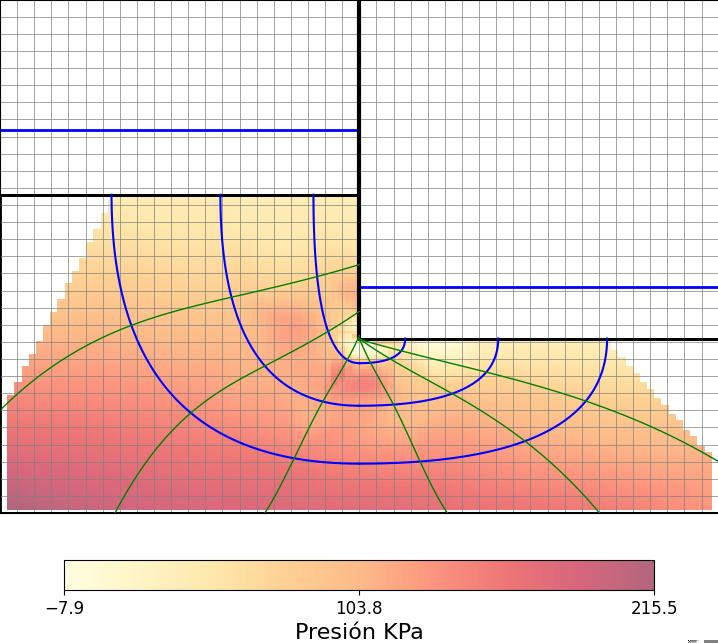
\includegraphics[width=\textwidth]{GRAFICOS/caso_1_presion_poros.jpg}
        \caption{Caso 1 Presion Poros}
    \end{minipage}
    \begin{minipage}{0.32\textwidth}
        \centering
        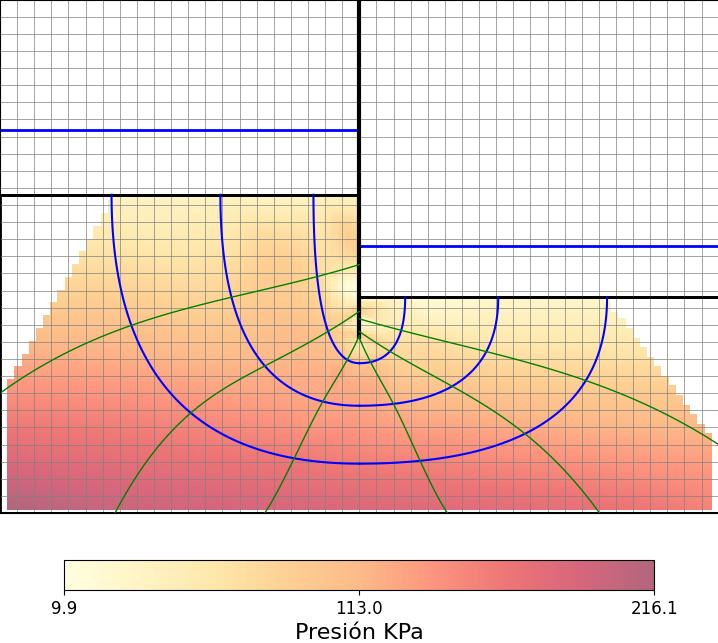
\includegraphics[width=\textwidth]{GRAFICOS/caso_2_presion_poros.jpg}
        \caption{Caso 2 Presion Poros}
    \end{minipage}
    \begin{minipage}{0.32\textwidth}
        \centering
        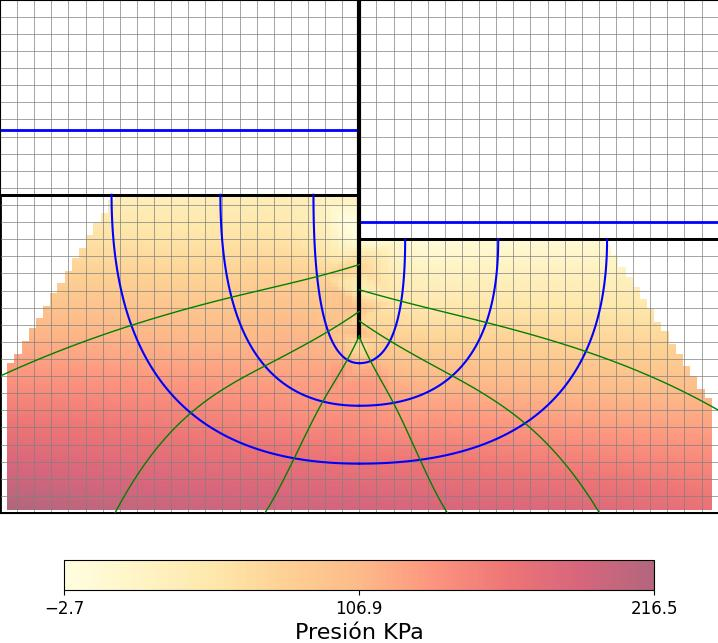
\includegraphics[width=\textwidth]{GRAFICOS/caso_3_presion_poros.jpg}
        \caption{Caso 3 Presion Poros}
    \end{minipage}
\end{figure}

\subsubsection{Presiones Totales}

\begin{figure}[H]
    \centering
    \begin{minipage}{0.32\textwidth}
        \centering
        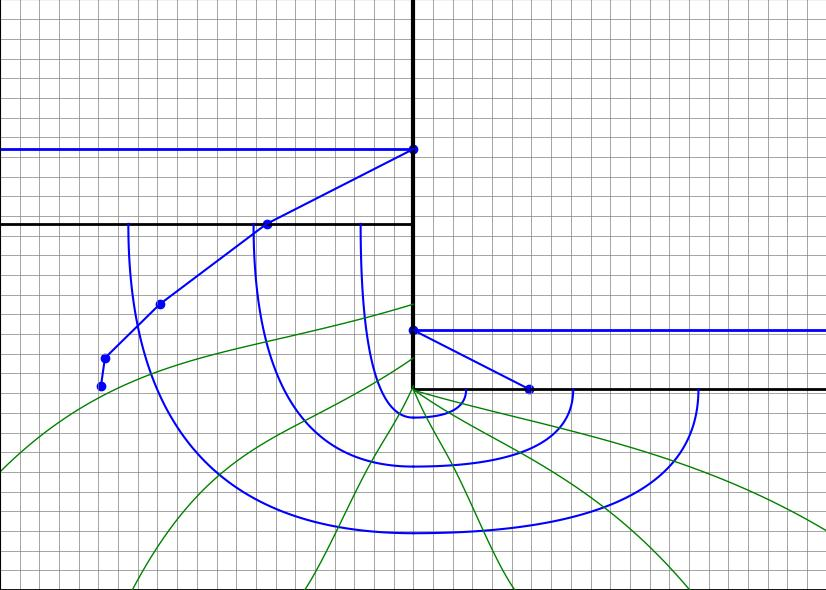
\includegraphics[width=\textwidth]{GRAFICOS/caso_1_presion_ataguia_total.jpg}
        \caption{Caso 1 Presion Ataguia Total}
    \end{minipage}
    \begin{minipage}{0.32\textwidth}
        \centering
        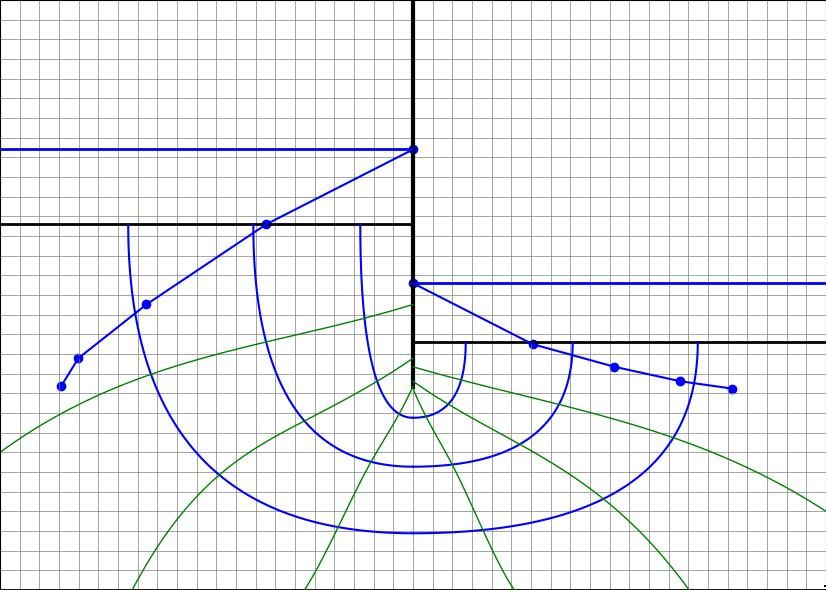
\includegraphics[width=\textwidth]{GRAFICOS/caso_2_presion_ataguia_total.jpg}
        \caption{Caso 2 Presion Ataguia Total}
    \end{minipage}
    \begin{minipage}{0.32\textwidth}
        \centering
        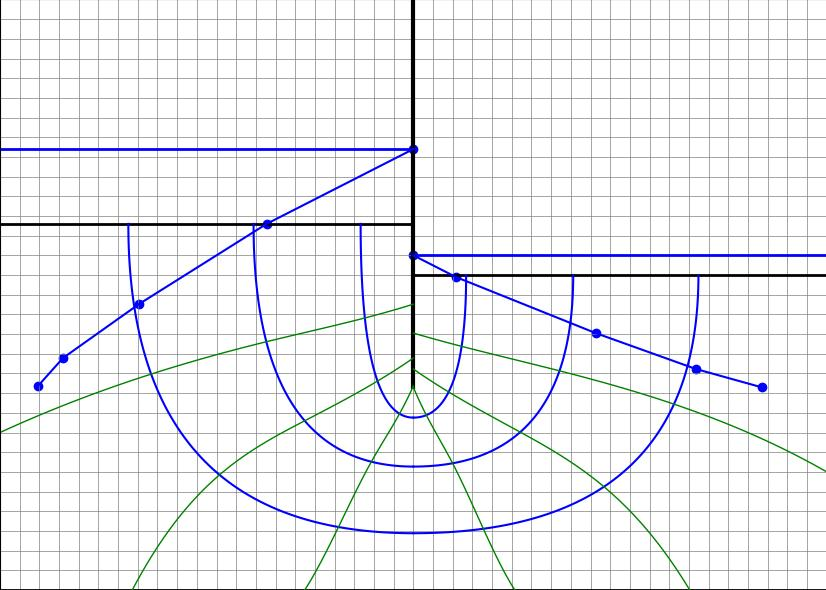
\includegraphics[width=\textwidth]{GRAFICOS/caso_3_presion_ataguia_total.jpg}
        \caption{Caso 3 Presion Ataguia Total}
    \end{minipage}
\end{figure}

\subsubsection{Presiones Efectivas}

\begin{figure}[H]
    \centering
    \begin{minipage}{0.32\textwidth}
        \centering
        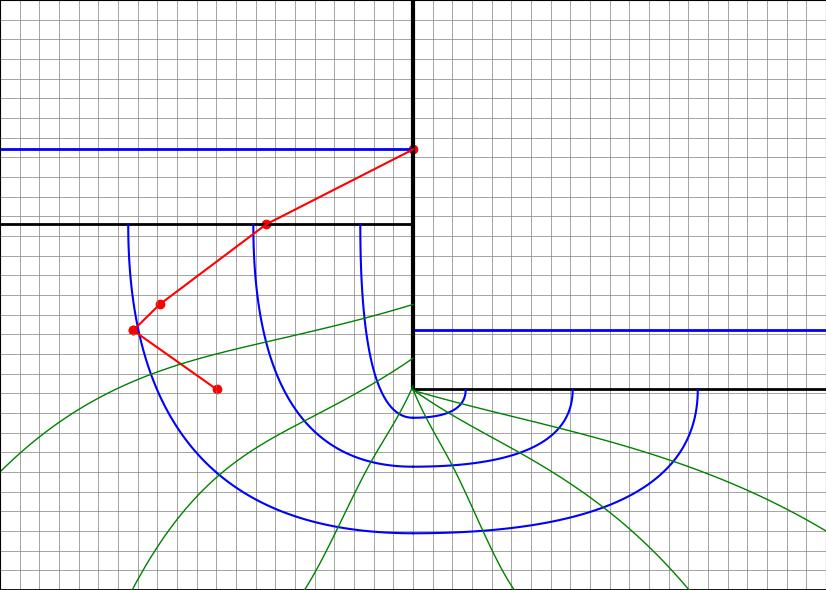
\includegraphics[width=\textwidth]{GRAFICOS/caso_1_presion_ataguia_neta.jpg}
        \caption{Caso 1 Presion Ataguia Neta}
    \end{minipage}
    \begin{minipage}{0.32\textwidth}
        \centering
        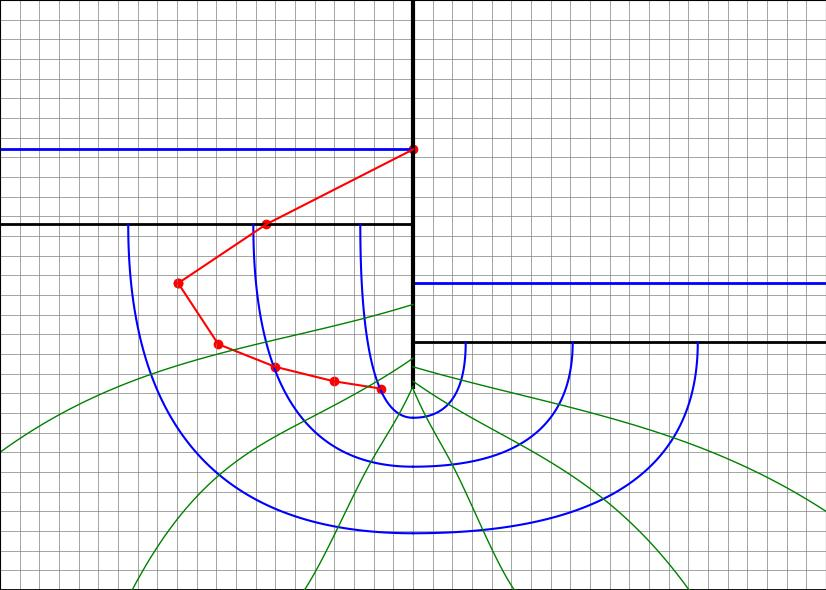
\includegraphics[width=\textwidth]{GRAFICOS/caso_2_presion_ataguia_neta.jpg}
        \caption{Caso 2 Presion Ataguia Neta}
    \end{minipage}
    \begin{minipage}{0.32\textwidth}
        \centering
        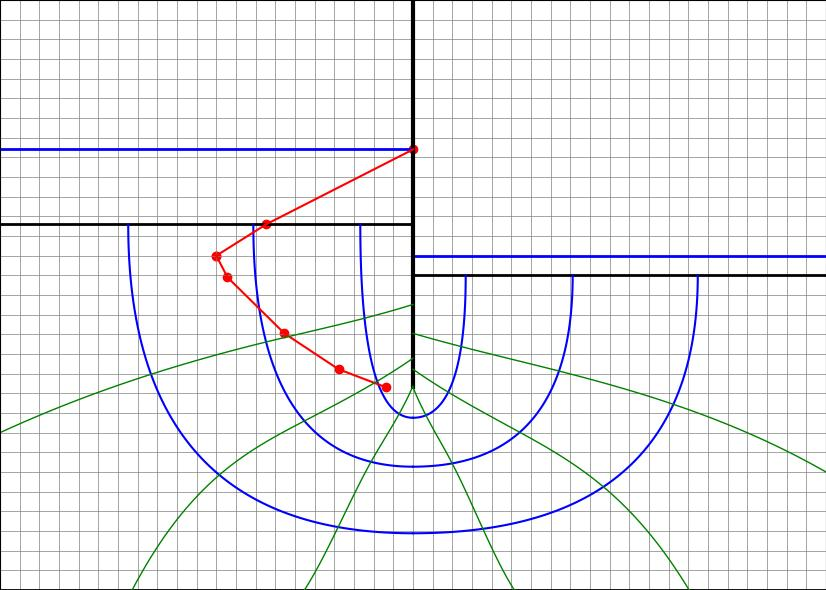
\includegraphics[width=\textwidth]{GRAFICOS/caso_3_presion_ataguia_neta.jpg}
        \caption{Caso 3 Presion Ataguia Neta}
    \end{minipage}
\end{figure}

\subsubsection{Estabilidad}

\begin{figure}[H]
    \centering
    \begin{minipage}{0.32\textwidth}
        \centering
        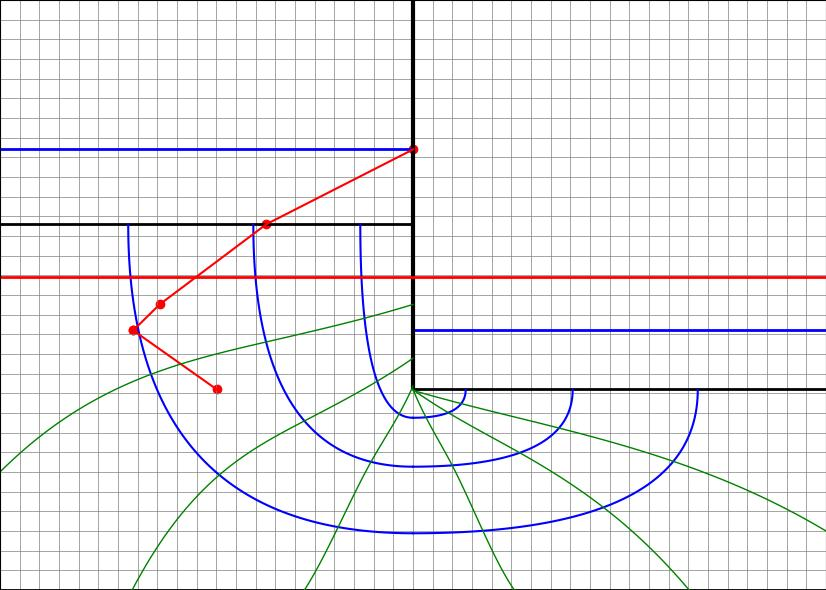
\includegraphics[width=\textwidth]{GRAFICOS/caso_1_centroide_y.jpg}
        \caption{Caso 1 Centroide}
    \end{minipage}
    \begin{minipage}{0.32\textwidth}
        \centering
        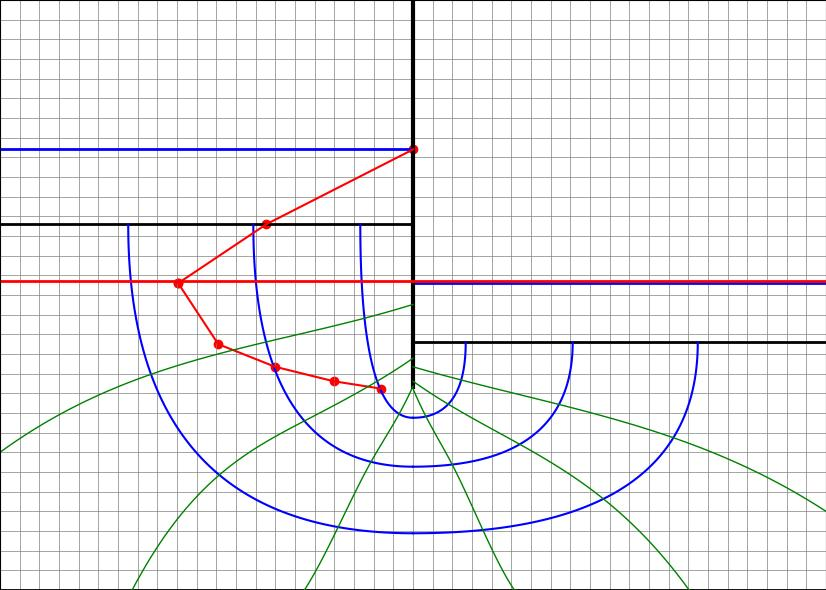
\includegraphics[width=\textwidth]{GRAFICOS/caso_2_centroide_y.jpg}
        \caption{Caso 2 Centroide}
    \end{minipage}
    \begin{minipage}{0.32\textwidth}
        \centering
        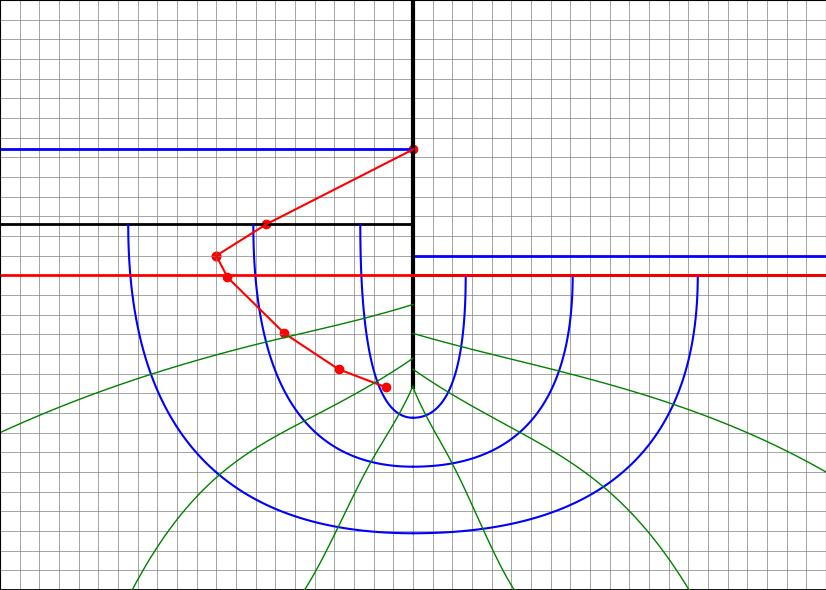
\includegraphics[width=\textwidth]{GRAFICOS/caso_3_centroide_y.jpg}
        \caption{Caso 3 Centroide}
    \end{minipage}
\end{figure}


\begin{table}[H]
    \begin{center}
        \caption{Gradientes hidraulicos y caudales obtenidos manualmente.}
        \begin{tabularx}{0.75\textwidth}{>{\centering\arraybackslash}X >{\centering\arraybackslash}X >{\centering\arraybackslash}X >{\centering\arraybackslash}X >{\centering\arraybackslash}X }\\
        \hline
        \boldmath{Propiedades} & \boldmath{Caso 1} & \boldmath{Caso 2} & \boldmath{Caso 3} & \boldmath{Unidades} \\
        \hline
        $i_{max}$ & $1.095$ & $0.629$ & $0.380$ & $-$ \\
        $i_{crit}$ & $1.141$ & $1.141$ & $1.141$ & $-$ \\
        $FS$ & $1.041$ & $1.811$ & $2.999$ & $-$\\
        $Q_{inf}$ & $43.877$ & $32.431$ & $25.754$ & $[\frac{m^3}{dia}]$\\
        \hline
        \end{tabularx}
        \label{tab:Manuales}
    \end{center}
\end{table}

\subsection{Resultados usando Diferencias Finitas}

\subsubsection{Caso 1}

\begin{figure}[H]
    \centering
    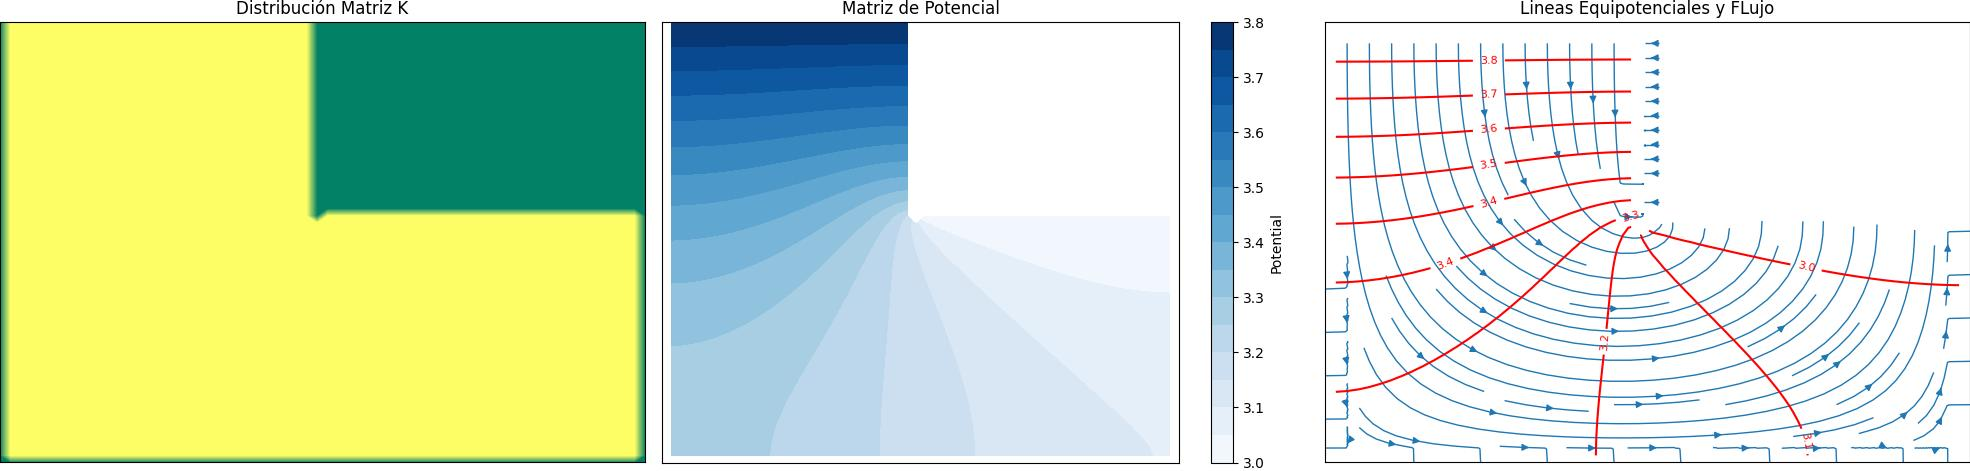
\includegraphics[width=\textwidth]{GRAFICOS/laplace_caso_1.jpg}
    \caption{Caso 1 Laplace}
\end{figure}

\subsubsection{Caso 2}

\begin{figure}[H]
    \centering
    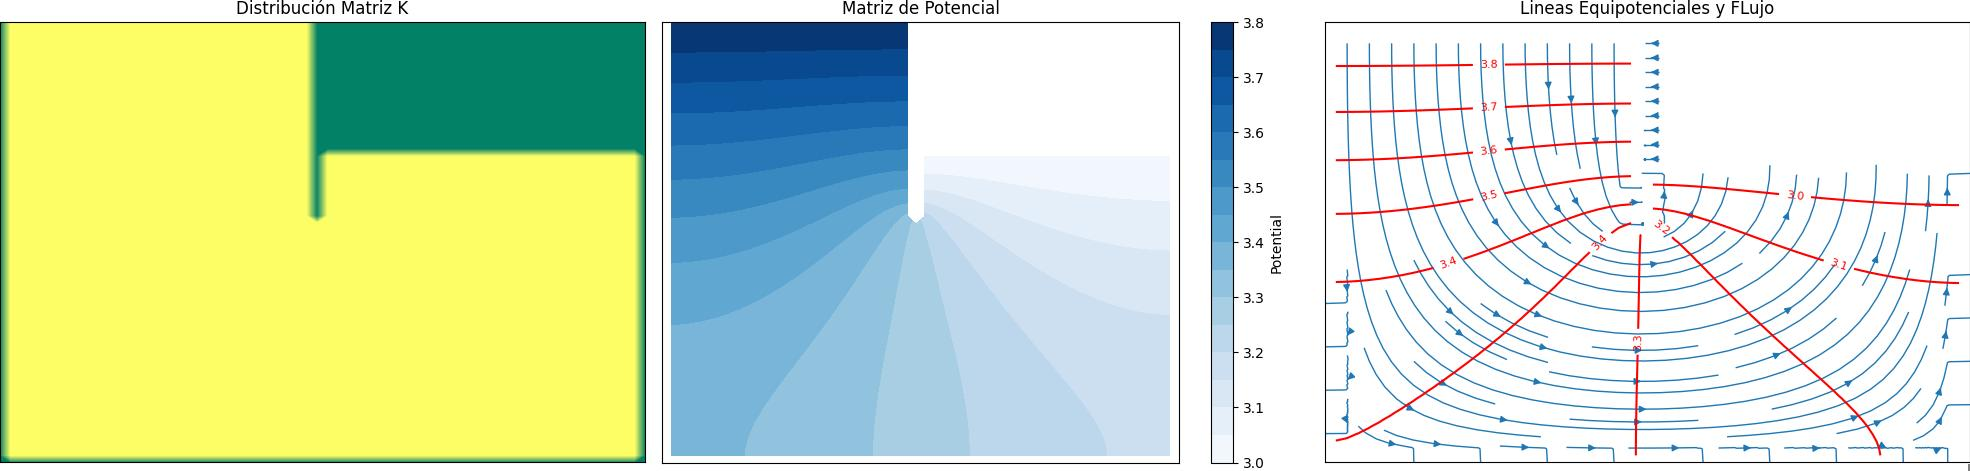
\includegraphics[width=\textwidth]{GRAFICOS/laplace_caso_2.jpg}
    \caption{Caso 2 Laplace}
\end{figure}

\subsubsection{Caso 3}

\begin{figure}[H]
    \centering
    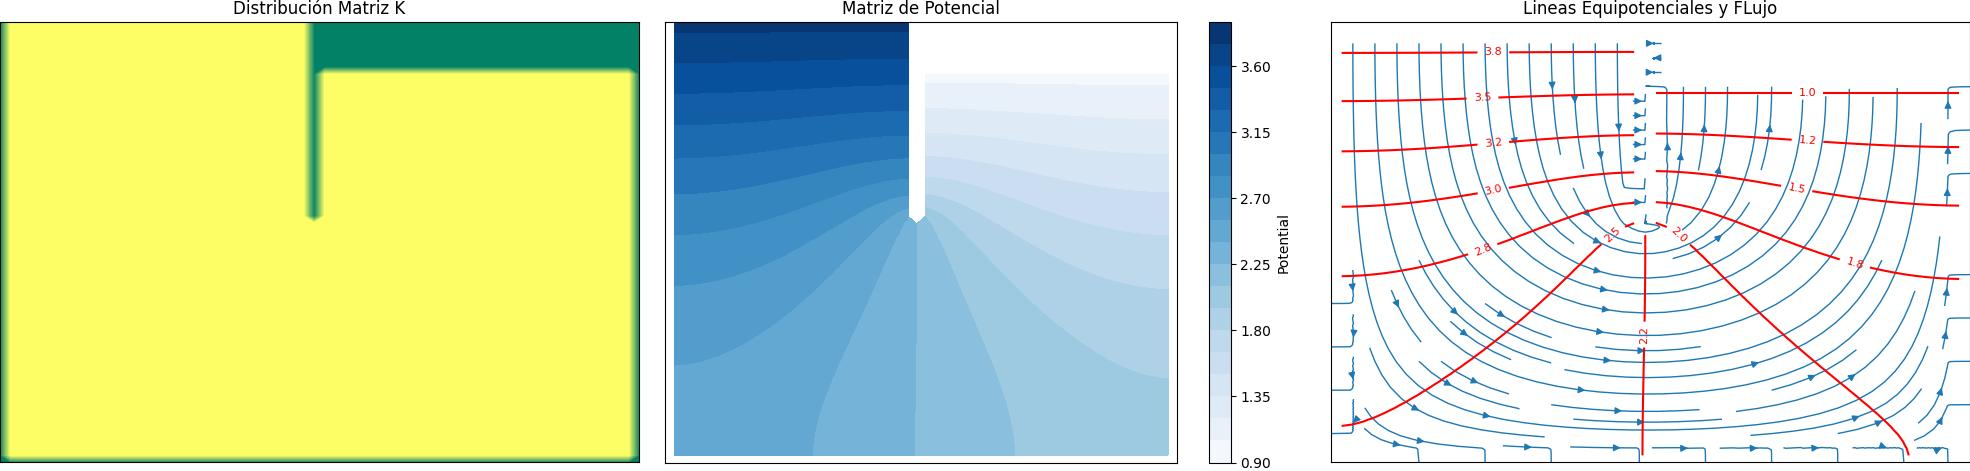
\includegraphics[width=\textwidth]{GRAFICOS/laplace_caso_3.jpg}
    \caption{Caso 3 Laplace}
\end{figure}

\begin{table}[H]
    \begin{center}
        \caption{Gradientes hidraulicos y caudales obtenidos mediante diferencias finitas.}
        \begin{tabularx}{0.75\textwidth}{>{\centering\arraybackslash}X >{\centering\arraybackslash}X >{\centering\arraybackslash}X >{\centering\arraybackslash}X >{\centering\arraybackslash}X }\\
        \hline
        \boldmath{Propiedades} & \boldmath{Caso 1} & \boldmath{Caso 2} & \boldmath{Caso 3} & \boldmath{Unidades} \\
        \hline
        $i_{max}$ & $1.095$ & $0.629$ & $0.380$ & $-$ \\
        $i_{crit}$ & $1.141$ & $1.141$ & $1.141$ & $-$ \\
        $FS$ & $1.041$ & $1.811$ & $2.999$ & $-$\\
        $Q_{inf}$ & $25.410$ & $20.790$ & $13.860$ & $[\frac{m^3}{dia}]$\\
        \hline
        \end{tabularx}
        \label{tab:Diferencias}
    \end{center}
\end{table}

\subsection{Resultados Escalamiento}

